\documentclass[10pt,a4paper]{article}

% ─── Packages ─────────────────────────────────────────

\usepackage{fontspec}
\setmainfont{Times New Roman}

\usepackage[top=1.0cm,bottom=0.9cm,left=1.45cm,right=1.45cm]{geometry}

\usepackage{titlesec}
\usepackage{enumitem}
\usepackage{hyperref}
\usepackage{xcolor}
\usepackage{tabularx}
\usepackage{graphicx}
\usepackage{parskip}

% ─── Colors ───────────────────────────────────────────

\definecolor{primary}{RGB}{30,40,90}
\definecolor{namecolor}{RGB}{0,120,180}
\definecolor{accent}{RGB}{50,90,150}
\definecolor{rulecol}{RGB}{200,205,220}
\definecolor{gray}{RGB}{90,90,90}

\hypersetup{
    colorlinks=true,
    urlcolor=accent
}

\pagestyle{empty}
\setlength{\parskip}{0pt}

% ─── Section ──────────────────────────────────────────

\titleformat{\section}
    {\normalsize\bfseries\color{primary}}
    {}
    {0em}
    {}
    [\vspace{1pt}\textcolor{rulecol}{\titlerule[0.6pt]}\vspace{1pt}]

\titlespacing{\section}{0pt}{4pt}{2pt}

% ─── Entry ────────────────────────────────────────────

\newcommand{\entry}[3]{%
    \noindent
    \begin{tabularx}{\linewidth}{X r}
        \textbf{\color{primary}#1} &
        {\scriptsize\color{gray}#2}
    \end{tabularx}\\[-2pt]
    {\scriptsize\textit{\color{gray}#3}}
    \vspace{0.5pt}
}

% ─── Compact list ─────────────────────────────────────

\newenvironment{cvitems}{
    \begin{itemize}[
        leftmargin=1.1em,
        topsep=0pt,
        itemsep=0.3pt,
        parsep=0pt,
        partopsep=0pt
    ]
}{
    \end{itemize}
}

% ═════════════════════════════════════════════════════

\begin{document}

% ─── HEADER ───────────────────────────────────────────

\noindent
\begin{tabularx}{\linewidth}{@{}X r@{}}

\begin{minipage}[c]{\linewidth}

    {\LARGE\bfseries\color{namecolor} Ho Huynh Nhu}\\[1pt]

    {\large\bfseries\color{primary}
    ERP Statistics Staff}\\[2pt]

    {\scriptsize\color{gray}
    20/10/2003
    \enspace\textcolor{rulecol}{|}
    \enspace (+84) 367 503 477
    \enspace\textcolor{rulecol}{|}
    \enspace
    \href{mailto:hhnhu2003@gmail.com}{hhnhu2003@gmail.com}
    \enspace\textcolor{rulecol}{|}
    \enspace Ho Chi Minh City}\\[1pt]

    {\scriptsize
    \href{https://github.com/hohuynhnhu}
    {github.com/hohuynhnhu}
    \enspace\textcolor{rulecol}{|}
    \enspace
    \href{https://www.facebook.com/huynhnhu.ho.961}
    {facebook.com/huynhnhu.ho.961}
    }

\end{minipage}

&

\begin{minipage}[c]{2.1cm}
    \raggedleft
    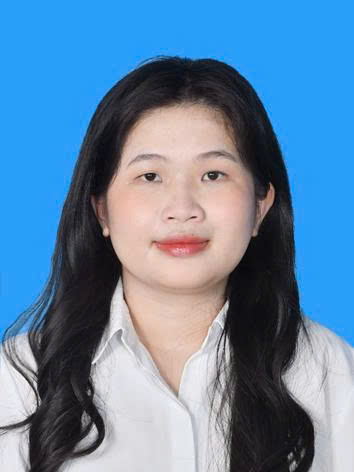
\includegraphics[
        width=2.1cm,
        height=2.5cm,
        keepaspectratio
    ]{assets/avt.jpg}
\end{minipage}

\end{tabularx}

\vspace{2pt}
\textcolor{rulecol}{\rule{\linewidth}{0.6pt}}

% ─── CAREER OBJECTIVE ─────────────────────────────────

\section*{Career Objective}

{\small
Final-year Information Technology student seeking an ERP Statistics Staff position. Experienced in working with business data from the Odoo ERP system: extracting, cleaning, validating, and aggregating data to produce accurate statistics and periodic reports with SQL, Excel, Python, and Power BI. Careful and responsible, with a strong focus on data accuracy and on automating repetitive reporting tasks to save time and keep figures up to date.
}

% ─── EDUCATION ────────────────────────────────────────

\section*{Education}

\entry
{University of Transport Ho Chi Minh City (UTH)}
{10/2022 -- 10/2026}
{Bachelor of Information Technology -- Completed coursework}

{\small
\begin{cvitems}
    \item GPA: \textbf{3.4 / 4.0}
    \item \textbf{Excellent Scholarship} -- Semester 1, 2025
    \item \textbf{Second Prize -- AI Track},
    UTH Student Scientific Research Conference 2025
\end{cvitems}
}

% ─── TECHNICAL SKILLS ─────────────────────────────────

\section*{Technical Skills}

{\small
\begin{tabularx}{\linewidth}{@{}lX@{}}

\textbf{ERP Data \& Statistics}
&
Odoo ERP business data, Data Extraction, Data Aggregation, Periodic Statistical Reports,
KPI Analysis, Data Validation \& Accuracy Checking
\\[1pt]

\textbf{Excel}
&
Pivot Table, Lookup Functions, Data Cleaning, Filtering, Summarizing, Reporting
\\[1pt]

\textbf{SQL / Databases}
&
SQL, PostgreSQL, SQL Server, MySQL, Joins, CTEs, Aggregations,
Subqueries, Window Functions
\\[1pt]

\textbf{BI / Visualization}
&
Power BI, DAX, Dashboard Development, Data Visualization, Operational Reporting
\\[1pt]

\textbf{Data Processing \& Automation}
&
Python, Pandas, NumPy, ETL/ELT, dbt, Apache Airflow
\\[1pt]

\textbf{Tools}
&
Git, Docker, Postman, VS Code, Jira, Confluence

\end{tabularx}
}

% ─── WORK EXPERIENCE ──────────────────────────────────

\section*{Work Experience}

\entry
{Gotik Consulting -- Data Engineer}
{Python \textbar{} dbt \textbar{} PostgreSQL \textbar{} Airflow \textbar{} Power BI}
{03/2026 -- 05/2026}

{\small
\begin{cvitems}
    \item Extracted, cleaned, and validated business data from the Odoo ERP system using Python and SQL, detecting discrepancies and preparing accurate, structured datasets for statistics and reporting.

    \item Built ETL pipelines to load processed data into Neon PostgreSQL, and automated hourly data workflows with Apache Airflow so that reports are always based on up-to-date data.

    \item Wrote SQL queries for aggregation, filtering, joins, and analytical reporting, cross-checking results to ensure reliable figures.

    \item Developed dbt models to standardize raw data into reusable analytical datasets, improving consistency across reports.

    \item Built Power BI dashboards and regular reports on operational and business metrics, helping management monitor performance.
\end{cvitems}
}

% ─── PROJECTS ─────────────────────────────────────────

\section*{Featured Data Projects}

\entry
{Delivery Driver -- Order Management \& Data Analytics System}
{Python \textbar{} PostgreSQL \textbar{} Kafka \textbar{} MinIO \textbar{} RFM \textbar{} Association Rule Mining}
{12/2025 -- 02/2026}

{\small
\begin{cvitems}
    \item Built an automated data pipeline with a Data Lake and Data Warehouse to collect, process, and prepare order data for statistical analysis.
    \item Applied RFM and Association Rule Mining to analyze customer orders and frequent pickup--delivery location pairs, generating insights to support business recommendations.
    \item GitHub: \href{https://github.com/LeKhang-cn22h/BE-delivery-driver}{BE-delivery-driver}
\end{cvitems}
}

\vspace{2pt}

\entry
{VehicleScan -- Smart Parking Data System}
{Python \textbar{} PostgreSQL \textbar{} Firebase \textbar{} ESP32 \textbar{} Kafka}
{03/2025 -- 03/2026}

{\small
\begin{cvitems}
    \item Collected and processed vehicle and IoT sensor data with Python and SQL, integrating AI, sensor, and application data into one centralized system for real-time monitoring and analysis.
    \item GitHub: \href{https://github.com/LeKhang-cn22h/VehicleScanner}{VehicleScanner}
\end{cvitems}
}

% ─── ADDITIONAL INFORMATION ───────────────────────────

\section*{Additional Information}

{\small

\begin{tabularx}{\linewidth}{@{}lX@{}}

\textbf{English}
&
Technical document reading and basic professional communication

\\[1pt]

\textbf{Working Style}
&
Careful, responsible, detail-oriented; proactive and quick to learn.

\\[1pt]

\textbf{Availability}
&
Available for full-time ERP Statistics Staff opportunities.

\end{tabularx}

}

\end{document}